%!TEX root=../main.tex
% Chapter Template

\chapter{Implementation} % Main chapter title

\label{Chapter5} % Change X to a consecutive number; for referencing this chapter elsewhere, use \ref{ChapterX}

%----------------------------------------------------------------------------------------
%	SECTION 1
%----------------------------------------------------------------------------------------
This chapter describes the design as it is implemented and hosted. It takes a look at the specifics of the product recommendation algorithm and provides implementation details.

\section{Solution overview}

The final solution consists of a \gls{REST} API build with ASP.NET Core and a MongoDB \gls{NoSQL} database. Both are hosted using Amazon Webservices in an EC2 instance using Docker. \\
The API consists of the commands seen in Appendix \ref{APICommands}. \\
This section covers the realization of the design derived from the requirements and the analysis.

\section{Creating the database}
The original data was in the form of SQL tables with a lot of attributes not neccessary for product recommendations. 
This data was transfered to MongoDB using a series of Python scripts. Only the data discovered in the design chapter was transfered. The Python scripts are attached with the source code.
To get a new client setup requires running many API calls or running the python scripts, in order to get the already acquired data to its No-SQL format.

\section{The product recommendation algorithm}
There are multiple ways to implement a product recommendation algorithm. The method chosen for this project is called Item-to-Item collaborative filtering. Other methods and the reasoning why these were not chosen is described in further detail in Chapter \ref{RelatedWork}. \\\\

Item-to-Item collaborative filtering is a data mining method to link items (products) with other items in terms of their similarity.
The specifics of the algorithm depends on the implementation. In this project each product is compared to other products based on how much they have been viewed together by customers, the likeness of their description and their product group. \\
The collaborative filter initially requires an exploration of each product. The visitors of each product are examined to discover what other products they have shown interest in. This uses a lot of resources, but after the first run only new behavior has to be re-calculated. Pseudo code of the algorithm can be seen in algorithm \ref{alg:collaborativeFilter}. At line 1 a for-loop is initiated, iterating through all products in the system. Line 2 prepares a dictionary where the similarity scores of the product will be stored. Line 3-11 loops through all visitors who have looked at the product. For each visitor (line 3) a loop is initiated looping through all products the visitor have looked at (line 4). In line 5 a check is made to see if the dictionary, containing the product similarity scores, already contain the product. If so, the score of that product is incremented by 1 (line 6). If not, the product is added to the dictionary (line 8). Once all the products that the visitor has shown interest in is looped through, the next visitor is examined. Once all visitors associated with the product are examined, the product scores are sorted descending (line 12). Once all products related to the product \textit{p} is found, the final similarity score is calculated for each of these products (line 13-15). Finally the product similarity scores are sorted descending and the top 10 most similar products to product \textit{p} are stored in the database (line 17-18), and the same procedure is done to the next product. The calculation of the similarity score can be seen in algorithm \ref{alg:calculateSimilarity}. The main product (\textit{p} from algorithm \ref{alg:collaborativeFilter}) is compared to a related product from \textit{productScores} calculated in algorithm \ref{alg:collaborativeFilter}. If the two products shares the same product group, the \textit{productGroupFactor} is set (line 4-6). Then the description of the two products are compared (line 8-12). For each word that matches in the two descriptions, the \textit{numOfSimAttributes} is incremented by 1. If there is no similar words in the two descriptions, the \textit{similarAttributeFactor} is set to 0. Finally the similarity score is calculated (line 16).\\\\

\begin{algorithm}[H]
\caption{Item-to-Item collaborative filtering algorithm}
\label{alg:collaborativeFilter}
\begin{algorithmic}[1]
\ForAll{Products p}
\State productScores = Dictionary<int, double>
\ForAll{Visitors in p}
\ForAll{Products visitorProduct in VisitorBehaviors}
\If{productScores contains visitorProduct}
\State productScores[visitorProduct]++
\Else
\State productScores.Add(visitorProduct, 1)
\EndIf
\EndFor
\EndFor
\State Sort productScores descending
\ForAll{Products relatedProduct in productScores}
\State productScores[relatedProduct] =
\State \textbf{calculateSimilarityScore(p, relatedProduct, productScores[relatedProduct])} (see algorithm \ref{alg:calculateSimilarity})
\EndFor
\State Sort productScores descending
\State Store top 10 productScores in database under p
\EndFor
\end{algorithmic}
\end{algorithm}

\begin{algorithm}[H]
\caption{Similarity calculations for two products }
\label{alg:calculateSimilarity}
\begin{algorithmic}[1]

\State \textbf{calculateSimilarityScore(mainProduct p1, compareProduct p2, currentScore)}
\State similarAttributeFactor = 0.02
\State productGroupFactor = 0
\State numOfSimAttributes = 0
\If{p1.productGroup equals p2.productGroup}
\State productGroupFactor = 0.02
\EndIf
\ForAll{words w in p1.description}
\If{w is in p2.description}
\State numOfSimAttributes++
\EndIf
\EndFor
\If{numOfSimAttributes equals 0}
\State similarAttributeFactor = 0
\EndIf
\State \textbf{return} \begin{math} currentScore * (1+productGroupFactor)*(1+similarAttributeFactor)^{numOfSimAttributes} \end{math}
\end{algorithmic}
\end{algorithm}

An overview of the process of generating a similarity score and storing it in the database can be seen in the flowchart in figure \ref{flowChartSimilarity}.

\begin{figure}[H]
\centering
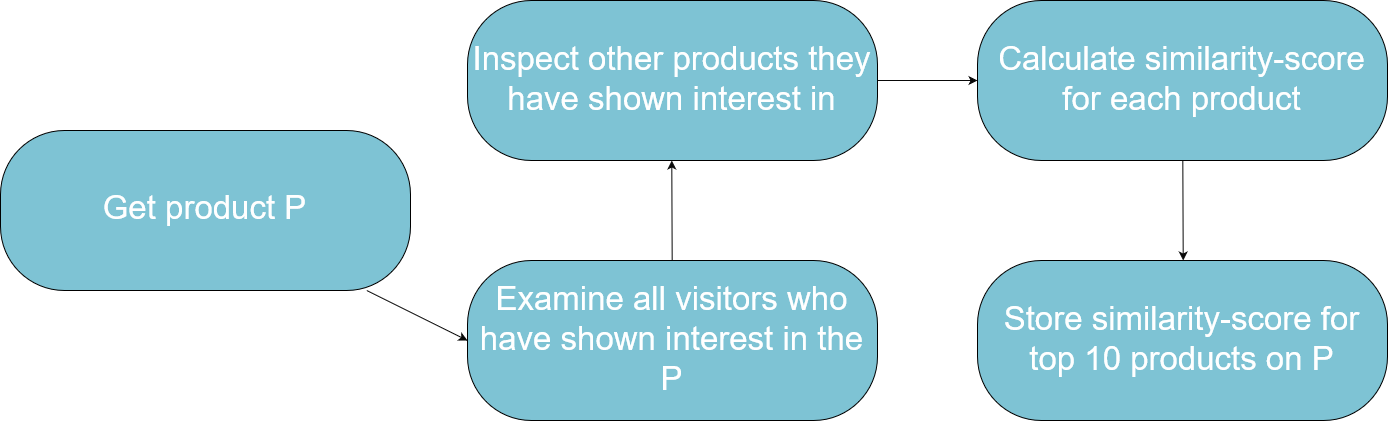
\includegraphics[scale=0.3]{FlowchartCalculateSimilarity}
\caption{The process of generating a similarity score for a product}
\label{flowChartSimilarity}
\end{figure}

When algorithms \ref{alg:collaborativeFilter} and \ref{alg:calculateSimilarity} are completed, each product in the database now has an array with the top 10 similar products based on amount of views, description and product group. \\
The next step is calculating the top products for each visitor. These are the products the specific visitor has viewed the most. This calculation can be seen in algorithm \ref{alg:topProducts}. In line 1 a loop is initiated, which iterates through each visitor. In line 2 a dictionary is prepared to contain all products the visitor have shown interest in as keys, and the amount of times he have looked at these as the value. Line 2-5 checks all behavior stored on the visitor (key of visitorProducts), and increment the value by 1. In line 6 the products are sorted descending, and the 5 products that the visitor have shown greatest interest in, is stored in the database (line 7). This calculation also requires a large amount of resources the first time, but very little to maintain.

\begin{algorithm}[H]
\caption{Calculations of each visitors top products}
\label{alg:topProducts}
\begin{algorithmic}[1]
\ForAll{Visitors v}
\State visitorProducts = Dictionary<string, int>
\ForAll{Behaviors b in v}
\State vistorProducts[b.Id]++
\EndFor
\State Sort visitorProducts descending
\State Store top 5 visitorProducts in database under v
\EndFor
\end{algorithmic}
\end{algorithm}

The process of recommending products is mainly a look-up in the database, since all these calculations are made before the actual product recommendations are requested. The pseudo code for the recommendation part can be seen in algorithm \ref{alg:recommendation}. The recommendation process starts with retrieving the requested visitor's top products from the database (line 1). In line 2 a dictionary is prepared to contain the final product recommendations. A for loop is initiated to iterate through all products \textit{p} in \textit{visitorTopProducts} (line 3). The similar products of the product \textit{p} is retrieved from the database (line 4). Each of these similar products are added to the \textit{productRecommendations} dictionary with their similarity score, or added to the summarized score if it already exists (line 6-9). Finally \textit{productRecommendations} is sorted descending, and the requested amount of recommendations are returned (line 13-14). 

\begin{algorithm}[H]
\caption{Get product recommendations}
\label{alg:recommendation}
\begin{algorithmic}[1]
\State visitorTopProducts = db.GetTopProducts(visitorUID)
\State productRecommendations = Dictionary<int, double>
\ForAll{Products p in visitorTopProducts}
\State similarProducts = db.GetTopProductRecommendation(p)
\ForAll{products simProduct in similarProducts}
\If{productRecommendations contains simProduct}
\State productRecommendations[simProduct] += similarProducts[simProduct]
\Else
\State productRecommendations.add(simProduct, similarProducts[simProduct]
\EndIf
\EndFor
\EndFor
\State Sort productRecommendations descending
\State \textbf{return} amount of productRecommendations requested
\State 
\end{algorithmic}
\end{algorithm}

The flowchart in figure \ref{flowchartRecomm} shows the process of requesting product recommendations.

\begin{figure}[H]
\centering
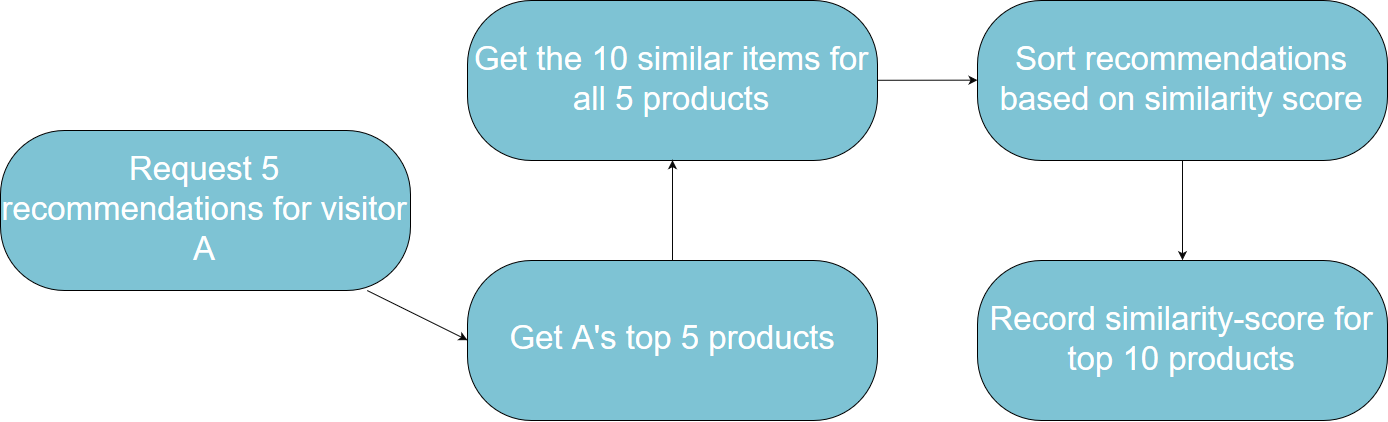
\includegraphics[scale=0.3]{FlowchatRequestRecomms}
\caption{The process of requesting 5 recommendations for visitor P}
\label{flowchartRecomm}
\end{figure}

The run time of the product recommendation part is examined below: \\
Visitors have a maximum of 5 top products, in the current implementation, which means the first for-loop has a maximum of 5 iterations. 
The second for-loop is at most 10 iterations, since each product can have no more than 10 similar items and.
Within the first for-loop is 1 constant operation of retrieving data from the database. The second for loop contains 1 constant addition operation.
The maximum of 5*10=50 product recommendations are sorted. Since the amount of products to be sorted cannot increase beyond 50 this is considered constant as well.
If the number of recommendations requested exceeds 50, products are added from the top 20 most popular products which is a maximum of 20 operations.
The final run time of the product recommendation algorithm is \\

\begin{math}
\centerline{ 5 * 1 * 10 * 1 * 50 * 20 = 50000}
\end{math}\\

50000 can seem like a large number, but it is a constant which means the algorithm runs in asymptotic time O(1). \\
The entire process of requesting product recommendations, running algorithm \ref{alg:recommendation} and returning them takes less than 40ms which satisfies the non-functional requirement NF02 - Efficiency. \\\\
When the visitor does not have enough or any behavior, recommendations are determined differently. In these cases the missing recommendations are retrieved from the top 20 most popular products in the last 30 days. The top 20 products are calculated by retrieving the behaviors from the last 30 days. The behaviors are iterated to see which products have the most views. The top 20 products are stored in the database and an API call will initiate the calculation.

\section{Handling new data}
When new visitors are created or new behavior is discovered the client has to call the corresponding API functions in order to store this data. When new behavior data is registered the program re-calculates the top products of the visitor along with the similar products of the product. This way the data is always up to date. The calculations can happen asynchronously and have no affect on the load times for the end user.

\section{Hosting the API}
The product recommendation API is hosted through Amazon WebServices in an \gls{EC2Instance} \cite{EC2}. The ASP.NET core project is built in a Docker container, the container is pushed to the Docker Hub and then pulled and run in the \gls{EC2Instance}. Docker is a tool that can be used to deploy applications within software containers. When a project is wrapped in a \gls{DockerContainer}, all necessary files from the system environment are wrapped as well. Docker itself is based off the Linux kernel, and can be deployed on any Linux server \cite{Docker}.  The database is similarly packed in a docker container and run in the \glspl{EC2Instance}. The Docker containers have exposed ports to the rest of the internet and can be accessed via \gls{EC2Instance} public DNS or IP.  Docker makes changing hosting platforms trivial since the container can be deployed without worrying about environment variables.



			


 